\chapter{Конструкторская часть}

В этом разделе будут представлены схемы алгоритмов классического умножения матриц, Винограда и его оптимизации.

\section{Разработка алгоритмов}

На рисунках~\ref{img:vinograd1}~---~\ref{img:vinogradopt3} представлены схемы алгоритмов классического умножения матриц, Винограда и его оптимизации.

\inputPdf{classic}{Схема алгоритма классического умножения матриц}

\inputPdf{vinograd1}{Схема алгоритма Винограда (часть 1)}

\begin{figure}[H]
	\center{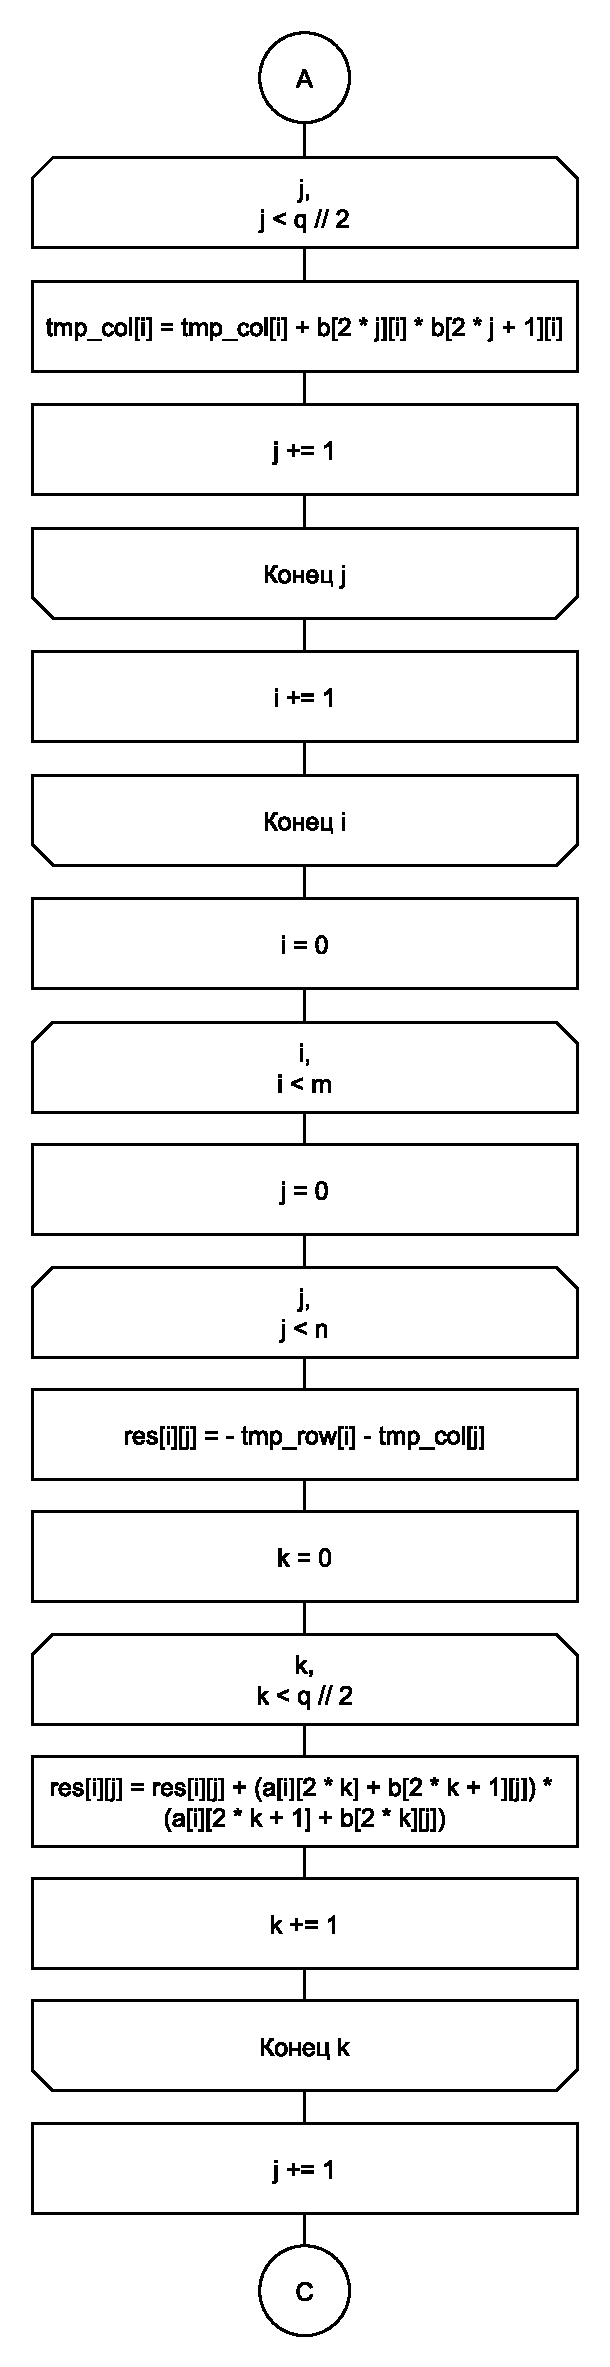
\includegraphics[width=0.38\textwidth]{img/vinograd2}}
	\caption{Схема алгоритма Винограда (часть 2)}
	\label{img:vinograd2}
\end{figure}

\inputPdf{vinograd3}{Схема алгоритма Винограда (часть 3)}

\inputPdf{vinogradopt1}{Схема оптимизированного алгоритма Винограда (часть 1)}

\begin{figure}[H]
	\center{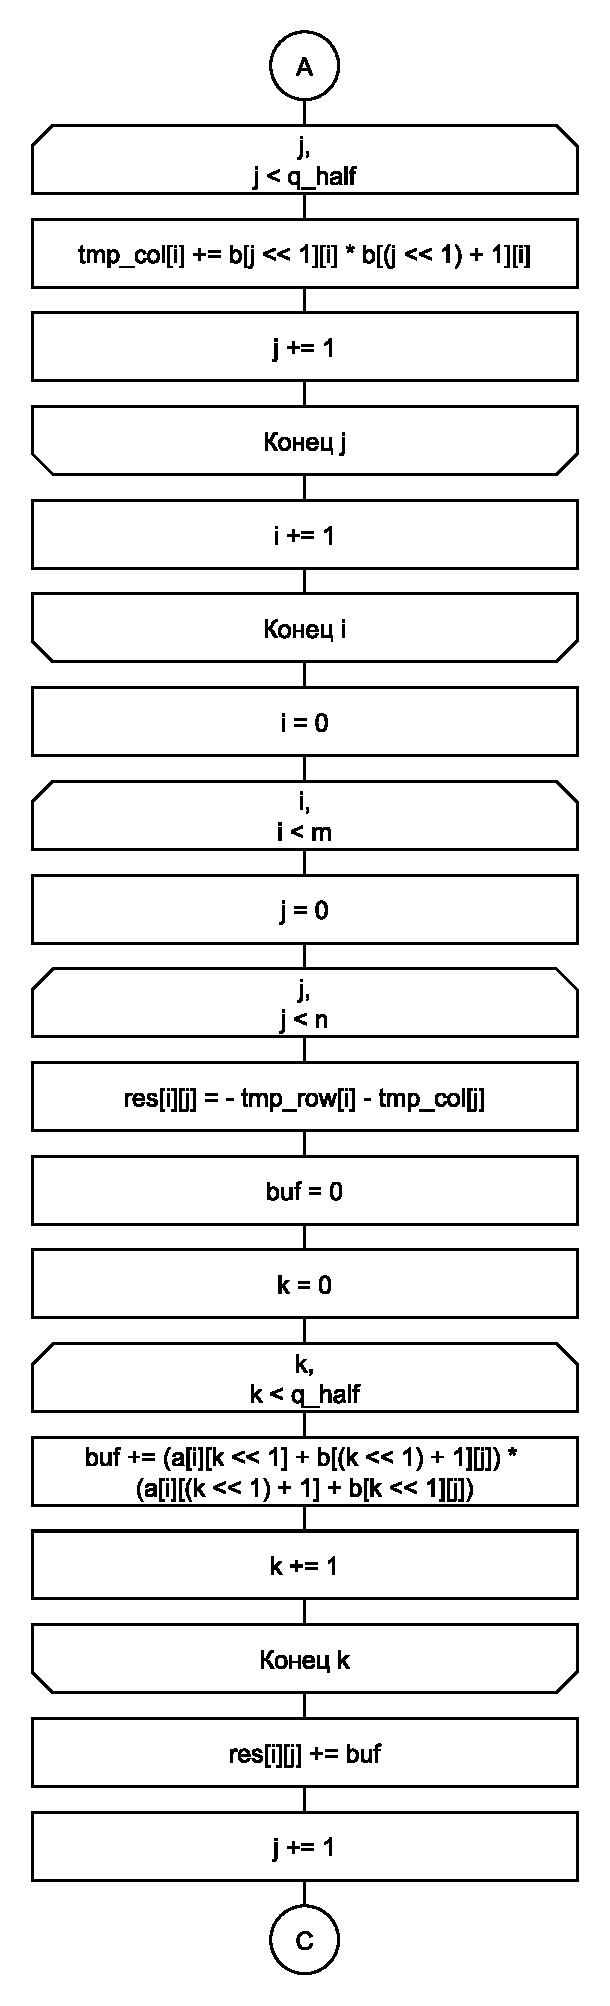
\includegraphics[width=0.45\textwidth]{img/vinogradopt2}}
	\caption{Схема оптимизированного алгоритма Винограда (часть 2)}
	\label{img:vinogradopt2}
\end{figure}

\inputPdf{vinogradopt3}{Схема оптимизированного алгоритма Винограда (часть 3)}

\section{Модель вычислений}

\begin{enumerate}
	\item Трудоемкость базовых операций.
	
	Следующие операторы имеют трудоемкость 1:
	$$+, -, +=, -=, =, ==, !=, >=, <=, >, <,$$
	$$>>, <<, [], \&, |, \&\&, ||, ++, --$$
	
	Следующие операторы имеют трудоемкость 2:
	$$*, /, \%, *=, /=$$
	
	\item Условный оператор.
	
	Для конструкций вида:
	\begin{lstlisting}
if (условие)
{
	Блок 1;
}
else
{
	Блок 2;
}
	\end{lstlisting}
	Пусть трудоемкость блока 1 --- $f_1$, блока 2 --- $f_2$. Пусть также трудоемкость условного перехода --- 0.
	
	Тогда трудоемкость условного оператора:
	\begin{equation}
		f_{if} = f_\textup{вычисления условия} + 
		\left[ \begin{gathered}
			\min(f_1, f_2), \textup{лучший случай}\\
			\max(f_1, f_2), \textup{худший случай}
		\end{gathered}
		\right.
	\end{equation}
	
	\item Трудоемкость циклов.
	
	Трудоемкость циклов вычисляется по следующей формуле:
	
	\begin{equation}
	\begin{aligned}
		f_\textup{цикла} =& f_\textup{инициализации} + f_\textup{сравнения} + \\
		& + M_\textup{шагов} \cdot (f_\textup{тела} + f_\textup{инкремента} + f_\textup{сравнения})
	\end{aligned}
	\end{equation}
	
\end{enumerate}

\section{Трудоемкость алгоритмов}

Рассчитаем трудоемкость алгоритмов умножения матриц.

\subsection{Классический алгоритм}

Трудоемкость классического алгоритма умножения матриц:

\begin{equation}
	\begin{aligned}
		f_\textup{классический} &= f_\textup{инициализации} + f_\textup{сравнения} + M \cdot (f_\textup{инкремента}+ f_\textup{сравнения} +\\
		&+ f_\textup{инициализации} + f_\textup{сравнения} + N \cdot (f_\textup{инкремента}+ f_\textup{сравнения} +\\ 
		&+f_\textup{инициализации} + f_\textup{сравнения} + Q\cdot(f_\textup{инкремента}+ f_\textup{сравнения}+\\
		&+ f_{[]} + f_{[]} + f_{=} + f_{[]} + f_{[]} + f_{+} + f_{[]} + f_{[]} + f_{*} + f_{[]} + f_{[]}))) =\\ 
		&= 1 +1 + M\cdot(1 +1 +1 +1 + N\cdot(1 +1 +1 +1 + Q\cdot\\
		&\cdot(1 +1 +1 +1 +1 +1 +1 +1 +1 +1 +2 +1 +1))) =\\
		&= 14MNQ + 4MN + 4M + 2
	\end{aligned}
\end{equation}

\subsection{Алгоритм Винограда}

Трудоемкость алгоритма Винограда будет складываться из следующих составляющих:
\begin{itemize}[label=---]
	\item вычисление слагаемых $- a_{i1}a_{i2} - a_{i3}a_{i4}$.
	\begin{equation}
	\begin{aligned}
		f_\RomanNumeralCaps{1} &= f_\textup{инициализации} + f_\textup{сравнения} + M \cdot (f_\textup{инкремента}+ f_\textup{сравнения} +\\
		&+ f_\textup{инициализации} + f_\textup{сравнения} + Q/2 \cdot (f_\textup{инкремента} + f_\textup{сравнения} +\\ 
		&+ f_{[]} +f_{=} + f_{[]} + f_{+} + f_{[]} + f_{*} + f_{[]} + f_{*} + f_{[]} + f_{*} + \\& + f_{+} + f_{[]}))=\\
		&= 1 + 1 + M\cdot(1 + 1 + 1+ 3 + Q/2\cdot(1 + 3 + 1 + 1 + 1 + 1 + \\
		&+ 1 + 2 + 1 + 2 + 1 + 2 + 1 + 1))=\\
		&= \frac{19MQ}{2} + 6M + 2
	\end{aligned}
	\end{equation}
	
	\item вычисление слагаемых $- b_{1j}b_{2j} - b_{3j}b_{4j}$.
	
	Аналогично получим:
	\begin{equation}
		f_\RomanNumeralCaps{2} = \frac{19NQ}{2} + 6N + 2
	\end{equation}
	
	\item заполнение результирующей матрицы.
	\begin{equation}
		\begin{aligned}
			f_\RomanNumeralCaps{3} &= f_\textup{инициализации} + f_\textup{сравнения} + M \cdot (f_\textup{инкремента}+ f_\textup{сравнения} +\\
			&+ f_\textup{инициализации} + f_\textup{сравнения} + N\cdot(f_\textup{инкремента} + f_\textup{сравнения} +\\ 
			& + f_{[]} + f_{[]} + f_{=} + f_{-} + f_{[]} + f_{-} + f_{[]} + f_\textup{инициализации} +\\
			&+ f_\textup{сравнения} + Q/2\cdot(f_\textup{инкремента}+ f_\textup{сравнения} + f_{[]} + f_{[]} + f_{=} +\\
			&+ f_{[]} + f_{[]} + f_{+} + f_{[]} + f_{*} + f_{[]} + f_{+} + f_{*} + f_{+} + f_{[]} + f_{[]} +\\
			&+ f_{*} + f_{[]} + f_{*} + f_{+} + f_{[]} + f_{+} + f_{*} + f_{[]} + f_{[]}))) =\\
			&= 1 + 1 + M\cdot(1 + 1 + 1 + 1 + N\cdot(1 + 1 + 1 + 1 +\\
			&+ 1 + 1 + 1 + 1 + 1 + 1 + 3 + Q/2\cdot(1 + 3 + 1 +1 +1 +\\
			&+1 +1 +1 +1 +2 +1 +1 +2 +1 +1 +1 +2 +1 +2 +1 +\\
			&+1 +1 +2 +1 +1))) =\\
			&= 16MNQ + 13MN + 4M + 2
		\end{aligned}
	\end{equation}
	
	\item учет нечетного Q.
	\begin{equation}
	\label{formula:if}
	\begin{aligned}
		f_\RomanNumeralCaps{4} &= f_\textup{условия} + 
		\left[ \begin{gathered}
			\min(f_1, f_2), \textup{лучший случай}\\
			\max(f_1, f_2), \textup{худший случай}
		\end{gathered}
		\right.
	\end{aligned}
	\end{equation}
	
	\begin{equation}
	\begin{aligned}
		f_\textup{условия} &= f_{\%} + f_{==} = \\
		&= 2 + 1 = 3
	\end{aligned}
	\end{equation}
	
	\begin{equation}
	\begin{aligned}
		f_1 &=  f_\textup{инициализации} + f_\textup{сравнения} + M \cdot (f_\textup{инкремента}+ f_\textup{сравнения} +\\
		&+ f_\textup{инициализации} + f_\textup{сравнения} + N \cdot (f_\textup{инкремента} + f_\textup{сравнения} +\\
		&+f_{[]} +f_{[]} +f_{=} +f_{[]} +f_{[]} +f_{+} +f_{[]} +f_{-} +f_{[]} +f_{*} +f_{-} +\\
		&+f_{[]} +f_{[]} =\\
		&= 1 + 1 + M\cdot(1 + 1 + 1 + 1 + N\cdot(1 + 1 + 1 +1 +1 +1 +1 +\\
		&+1 +1 +1 +1 +2 +1 +1 +1)) =\\
		&= 16MN + 4M + 2
	\end{aligned}
	\end{equation}
	
	\begin{equation}
		f_2 = 0
	\end{equation}
	
	Тогда формула~\ref{formula:if} примет вид:
	\begin{equation}
	\begin{aligned}
		f_\RomanNumeralCaps{4} = 3 + 
		\left[ \begin{aligned}
			&0, \textup{лучший случай: Q четное}\\
			&16MN + 4M + 2, \textup{худший случай: Q нечетное}
		\end{aligned}
		\right.
	\end{aligned}
	\end{equation}
\end{itemize}

Таким образом, трудоемкость алгоритма Винограда:
	\begin{equation}
	\begin{aligned}
		f_\textup{Виноград} &= f_\RomanNumeralCaps{1} + f_\RomanNumeralCaps{2} + f_\RomanNumeralCaps{3} + f_\RomanNumeralCaps{4} =\\
		&= \frac{19MQ}{2} + 6M + 2 + \frac{19NQ}{2} + 6N + 2 + 16MNQ +\\ 
		&+13MN + 4M + 2 + 3 + \\
		&+\left[ \begin{aligned}
			&0, \textup{лучший случай: Q четное}\\
			&16MN + 4M + 2, \textup{худший случай: Q нечетное}
		\end{aligned}
		\right. =\\
		&= \frac{19MQ}{2} + \frac{19NQ}{2} + 16MNQ + 13MN + 10M + 6N + 9
	\end{aligned}
	\end{equation}

\subsection{Оптимизированный алгоритм Винограда}

Трудоемкость оптимизированного алгоритма Винограда будет складываться из следующих составляющих:

\begin{itemize}[label=---]
	\item предвычисление $q//2$.
	
	\begin{equation}
		f_\textup{пред} = 2
	\end{equation}
	
	\item вычисление слагаемых $- a_{i1}a_{i2} - a_{i3}a_{i4}$.
	\begin{equation}
		\begin{aligned}
			f_\RomanNumeralCaps{1} &= f_\textup{инициализации} + f_\textup{сравнения} + M \cdot (f_\textup{инкремента}+ f_\textup{сравнения} +\\
			&+ f_\textup{инициализации} + f_\textup{сравнения} + Q/2 \cdot (f_\textup{инкремента} + f_\textup{сравнения} +\\ 
			&+ f_{[]} +f_{+=} + f_{[]} + f_{<<} + f_{[]} + f_{*} + f_{[]} + f_{<<} + \\& + f_{+} + f_{[]}))=\\
			&= 1 + 1 + M\cdot(1 + 1 + 1+ 1 + Q/2\cdot(1 + 1 + 1 + 1 + 1 + 1 + \\
			&+ 1 + 2 + 1 + 1 + 1 + 1))=\\
			&= \frac{13MQ}{2} + 4M + 2
		\end{aligned}
	\end{equation}
	
	\item вычисление слагаемых $- b_{1j}b_{2j} - b_{3j}b_{4j}$.
	
	Аналогично получим:
	\begin{equation}
		f_\RomanNumeralCaps{2} = \frac{13NQ}{2} + 4N + 2
	\end{equation}
	
	\item заполнение результирующей матрицы.
	\begin{equation}
		\begin{aligned}
			f_\RomanNumeralCaps{3} &= f_\textup{инициализации} + f_\textup{сравнения} + M \cdot (f_\textup{инкремента}+ f_\textup{сравнения} +\\
			&+ f_\textup{инициализации} + f_\textup{сравнения} + N\cdot(f_\textup{инкремента} + f_\textup{сравнения} +\\ 
			& + f_{[]} + f_{[]} + f_{=} + f_{-} + f_{[]} + f_{-} + f_{[]} + f_{=} + f_\textup{инициализации} +\\
			&+ f_\textup{сравнения} + Q/2\cdot(f_\textup{инкремента}+ f_\textup{сравнения} +  f_{+=} + f_{[]}+\\
			&+ f_{<<} + f_{[]} + f_{+} + f_{<<} + f_{+} + f_{[]} + f_{[]} + f_{*} + f_{[]} + f_{<<}+\\
			& + f_{+} + f_{[]} + f_{+} + f_{<<} + f_{[]} + f_{[]}))) =\\
			&= 1 + 1 + M\cdot(1 + 1 + 1 + 1 + N\cdot(1 + 1 + 1 + 1 + 1 + 1 +\\
			&+ 1 + 1 + 1 + 1 + 1 + 1 + Q/2\cdot(1 + 1 + 1 +1 +1 +1 +1 +\\
			&+1 +1 +1 +1 +2 +1 +1 +1 +1 +1 +1 +1 +1))) =\\
			&= \frac{21MNQ}{2} + 12MN + 4M + 2
		\end{aligned}
	\end{equation}
	
	\item учет нечетного Q.
	\begin{equation}
		\label{formula:ifopt}
		\begin{aligned}
			f_\RomanNumeralCaps{4} &= f_\textup{условия} + 
			\left[ \begin{gathered}
				\min(f_1, f_2), \textup{лучший случай}\\
				\max(f_1, f_2), \textup{худший случай}
			\end{gathered}
			\right.
		\end{aligned}
	\end{equation}
	
	\begin{equation}
		\begin{aligned}
			f_\textup{условия} &= f_{\%} + f_{==} = \\
			&= 2 + 1 = 3
		\end{aligned}
	\end{equation}
	
	\begin{equation}
		\begin{aligned}
			f_1 &=  f_\textup{инициализации} + f_\textup{сравнения} + M \cdot (f_\textup{инкремента}+ f_\textup{сравнения} +\\
			&+ f_\textup{инициализации} + f_\textup{сравнения} + N \cdot (f_\textup{инкремента} + f_\textup{сравнения} +\\
			&+f_{[]} +f_{[]} +f_{+=} +f_{[]} +f_{-} +f_{[]} +f_{*} +f_{-} +\\
			&+f_{[]} +f_{[]} =\\
			&= 1 + 1 + M\cdot(1 + 1 + 1 + 1 + N\cdot(1 + 1 + 1 +1 +1 +\\ 
			&+1 +1 +1 +2 +1 +1 +1)) =\\
			&= 13MN + 4M + 2
		\end{aligned}
	\end{equation}
	
	\begin{equation}
		f_2 = 0
	\end{equation}
	
	Тогда формула~\ref{formula:ifopt} примет вид:
	\begin{equation}
		\begin{aligned}
			f_\RomanNumeralCaps{4} = 3 + 
			\left[ \begin{aligned}
				&0, \textup{лучший случай: Q четное}\\
				&13MN + 4M + 2, \textup{худший случай: Q нечетное}
			\end{aligned}
			\right.
		\end{aligned}
	\end{equation}
\end{itemize}

Таким образом, трудоемкость оптимизированного алгоритма Винограда:
\begin{equation}
	\begin{aligned}
		f_\textup{Виноград} &= f_\textup{пред} + f_\RomanNumeralCaps{1} + f_\RomanNumeralCaps{2} + f_\RomanNumeralCaps{3} + f_\RomanNumeralCaps{4} =\\
		&= 2 + \frac{13MQ}{2} + 4M + 2 + \frac{13NQ}{2} + 4N + 2 + \frac{21MNQ}{2} +\\
		&+ 12MN + 4M + 2 + 3+\\
		&+\left[ \begin{aligned}
			&0, \textup{лучший случай: Q четное}\\
			&13MN + 4M + 2, \textup{худший случай: Q нечетное}
		\end{aligned}
		\right. =\\
		&= \frac{21MNQ}{2} + \frac{13MQ}{2} + \frac{13NQ}{2} + 12MN + 8M + 4N + 11 +\\
		&+\left[ \begin{aligned}
			&0, \textup{лучший случай: Q четное}\\
			&13MN + 4M + 2, \textup{худший случай: Q нечетное}
		\end{aligned}
		\right.
	\end{aligned}
\end{equation}


\section{Классы эквивалентности тестирования}

Для тестирования выделены следующие классы эквивалентности:

\begin{enumerate}
	\item одна из матриц пустая;
	\item количество строк первой матрицы не равно количеству столбцов второй;
	\item умножение матриц с размерами $[1\times1]$;
	\item умножение квадратных матриц;
	\item умножение прямоугольных матриц.
\end{enumerate}

\section{Использование памяти}

\begin{enumerate}
	\item Классический алгоритм:
	\begin{itemize}[label=---]
		\item две входные матрицы: $M\cdot Q \cdot sizeof(int) + Q\cdot N \cdot sizeof(int)$;
		\item результирующая матрица: $M\cdot N\cdot sizeof(int)$;
		\item дополнительные переменные: $3\cdot sizeof(int)$.
	\end{itemize}
	
	Таким образом, необходимая память:
	\begin{equation}
		\label{memclassic}
		sizeof(int)\cdot(M(Q+N)+QN+3)
	\end{equation}
	
	\item Алгоритм Винограда:
	\begin{itemize}[label=---]
		\item две входные матрицы: $M\cdot Q \cdot sizeof(int) + Q\cdot N \cdot sizeof(int)$;
		\item результирующая матрица: $M\cdot N\cdot sizeof(int)$;
		\item массив-строка для слагаемых: $M\cdot sizeof(int)$;
		\item массив-столбец для слагаемых: $N\cdot sizeof(int)$;
		\item дополнительные переменные: $3\cdot sizeof(int)$.
	\end{itemize}
	
	Таким образом, необходимая память:
	\begin{equation}
		\label{mem}
		sizeof(int)\cdot(M(Q+N+1) + N(Q+1) + 3)
	\end{equation}
	
	\item Оптимизированный алгоритм Винограда:
	\begin{itemize}[label=---]
		\item две входные матрицы: $M\cdot Q \cdot sizeof(int) + Q\cdot N \cdot sizeof(int)$;
		\item результирующая матрица: $M\cdot N\cdot sizeof(int)$;
		\item массив-строка для слагаемых: $M\cdot sizeof(int)$;
		\item массив-столбец для слагаемых: $N\cdot sizeof(int)$;
		\item дополнительные переменные: $5\cdot sizeof(int)$.
	\end{itemize}
	
	Таким образом, необходимая память:
	\begin{equation}
		\label{memopt}
		sizeof(int)\cdot(M(Q+N+1) + N(Q+1) + 5)
	\end{equation}
\end{enumerate}

\section*{Вывод}

Сравнивая формулы~\ref{mem} и~\ref{memopt}, можно сделать вывод, что оптимизированный алгоритм Винограда требует больше памяти, чем классический: затраты на $2\cdot sizeof(int)$ байт больше. Но наименьшие затраты по памяти у классического алгоритма умножения матриц.

\section{Вывод}

В данном разделе были представлены схемы алгоритмов, рассматриваемых в лабораторной работе.